\clearpage\subsection{AMD enero 2022}
\begin{center}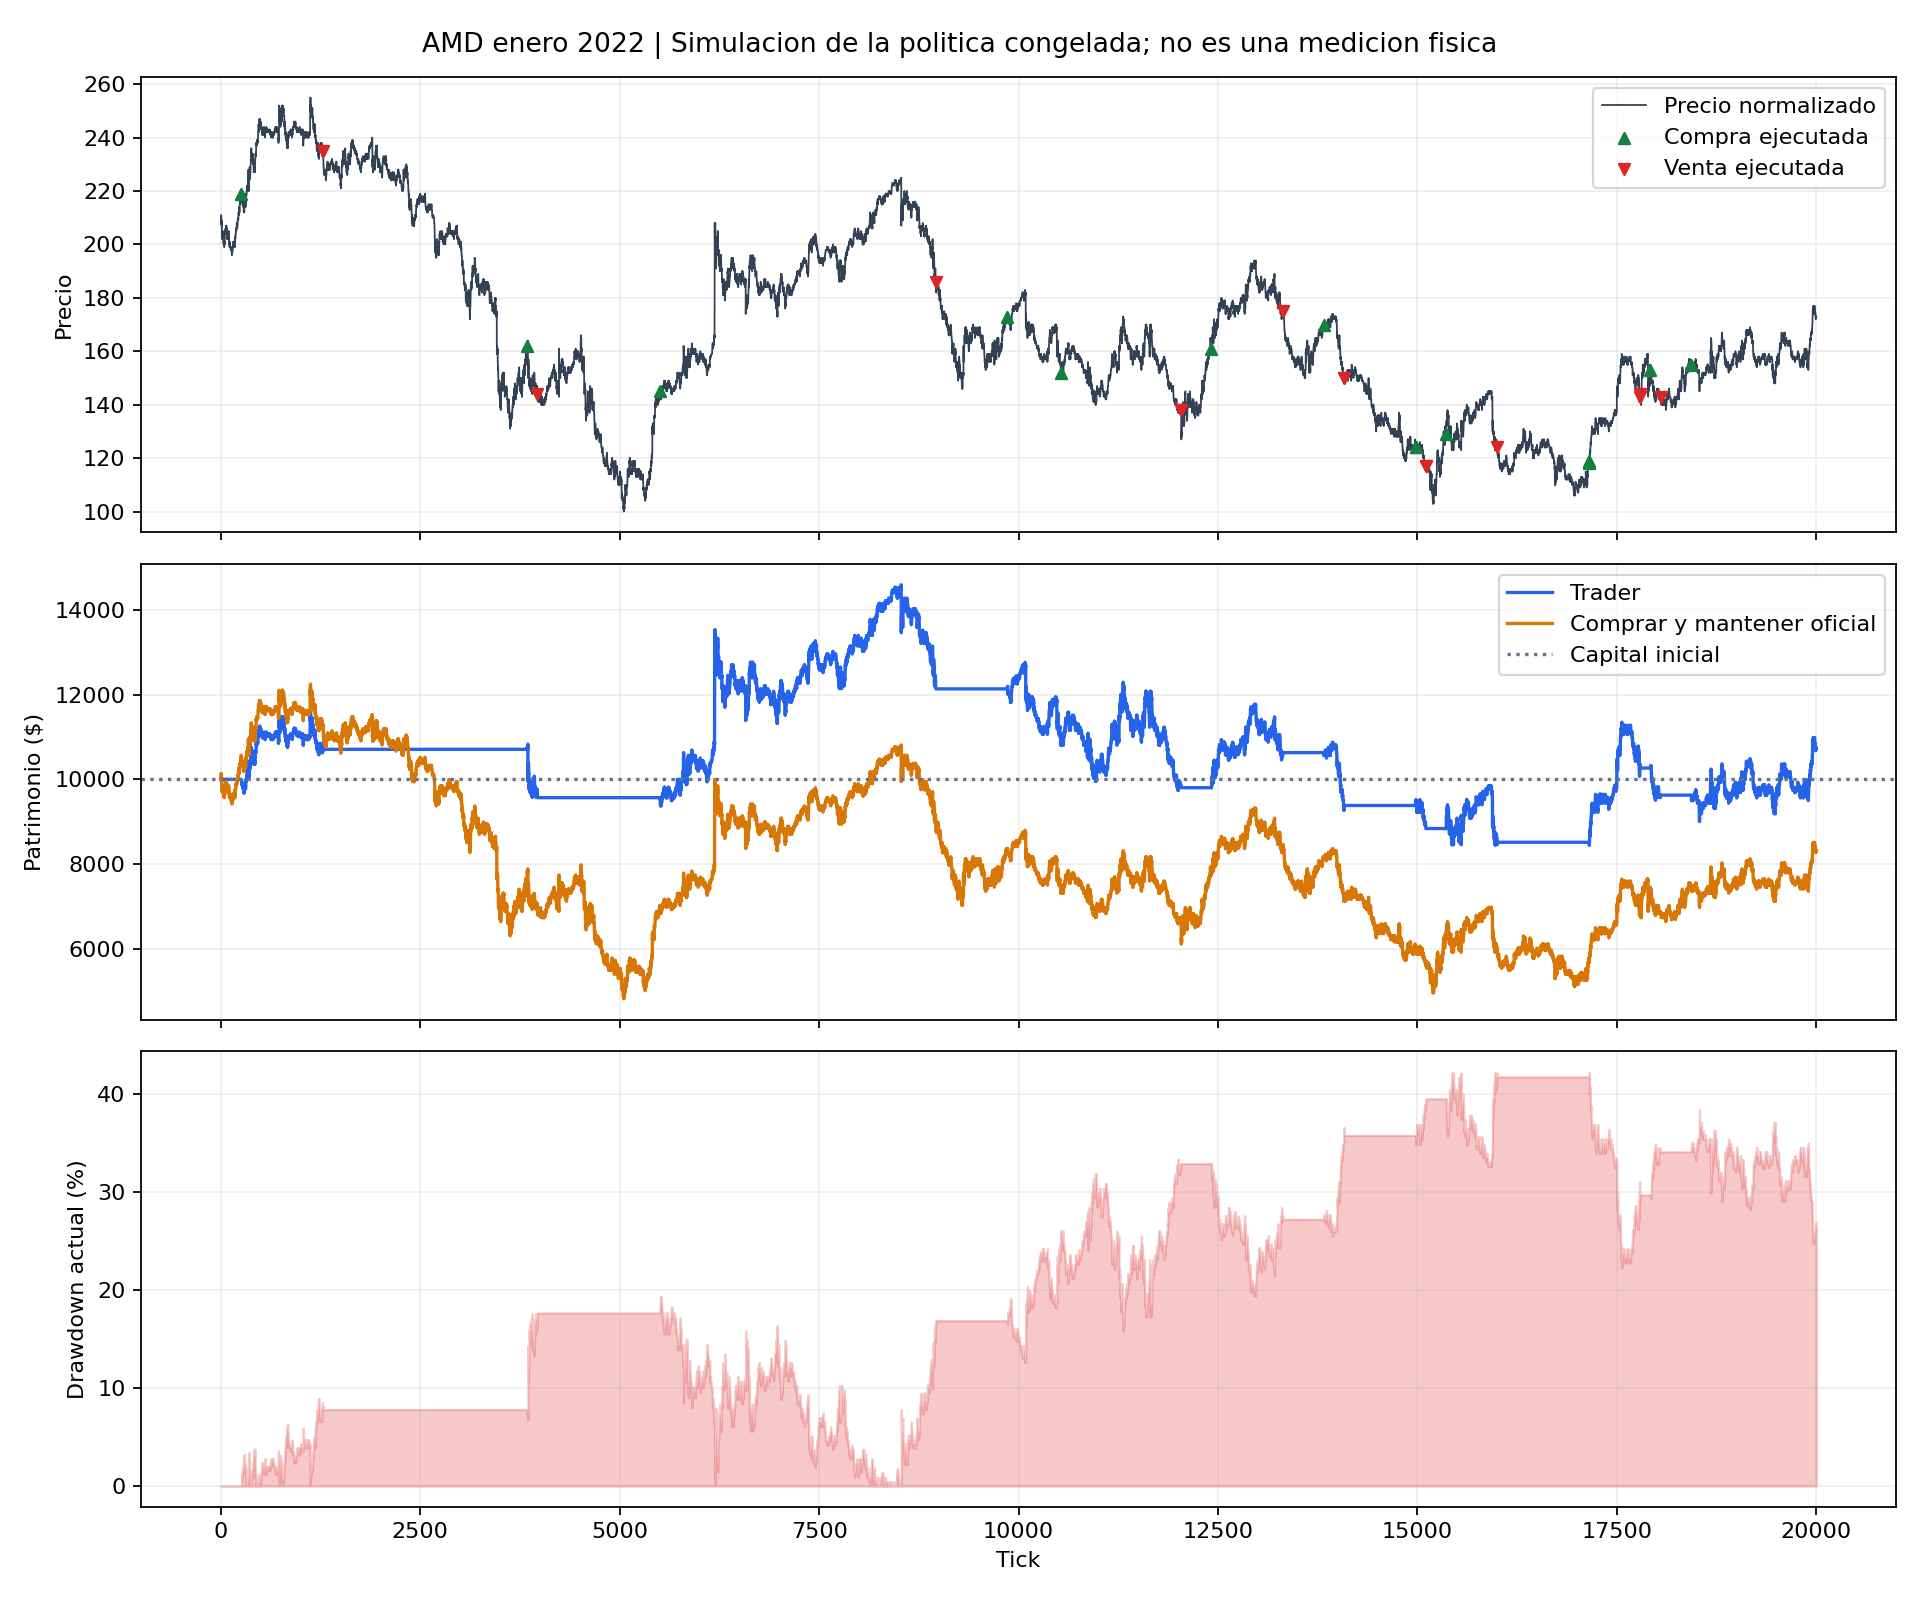
\includegraphics[width=\linewidth,height=0.70\textheight,keepaspectratio]{figuras/amd_enero.png}\end{center}
Trader: \$10\,738; mantener: \$8\,315; ventaja: \$2\,423. Órdenes: 27; comisiones: \$135; drawdown máximo: 42,20\%.

Los marcadores representan ejecuciones al precio siguiente al que generó la señal. Es simulación sobre datos conocidos; no es telemetría de la placa.

\clearpage\subsection{AMD mayo 2022}
\begin{center}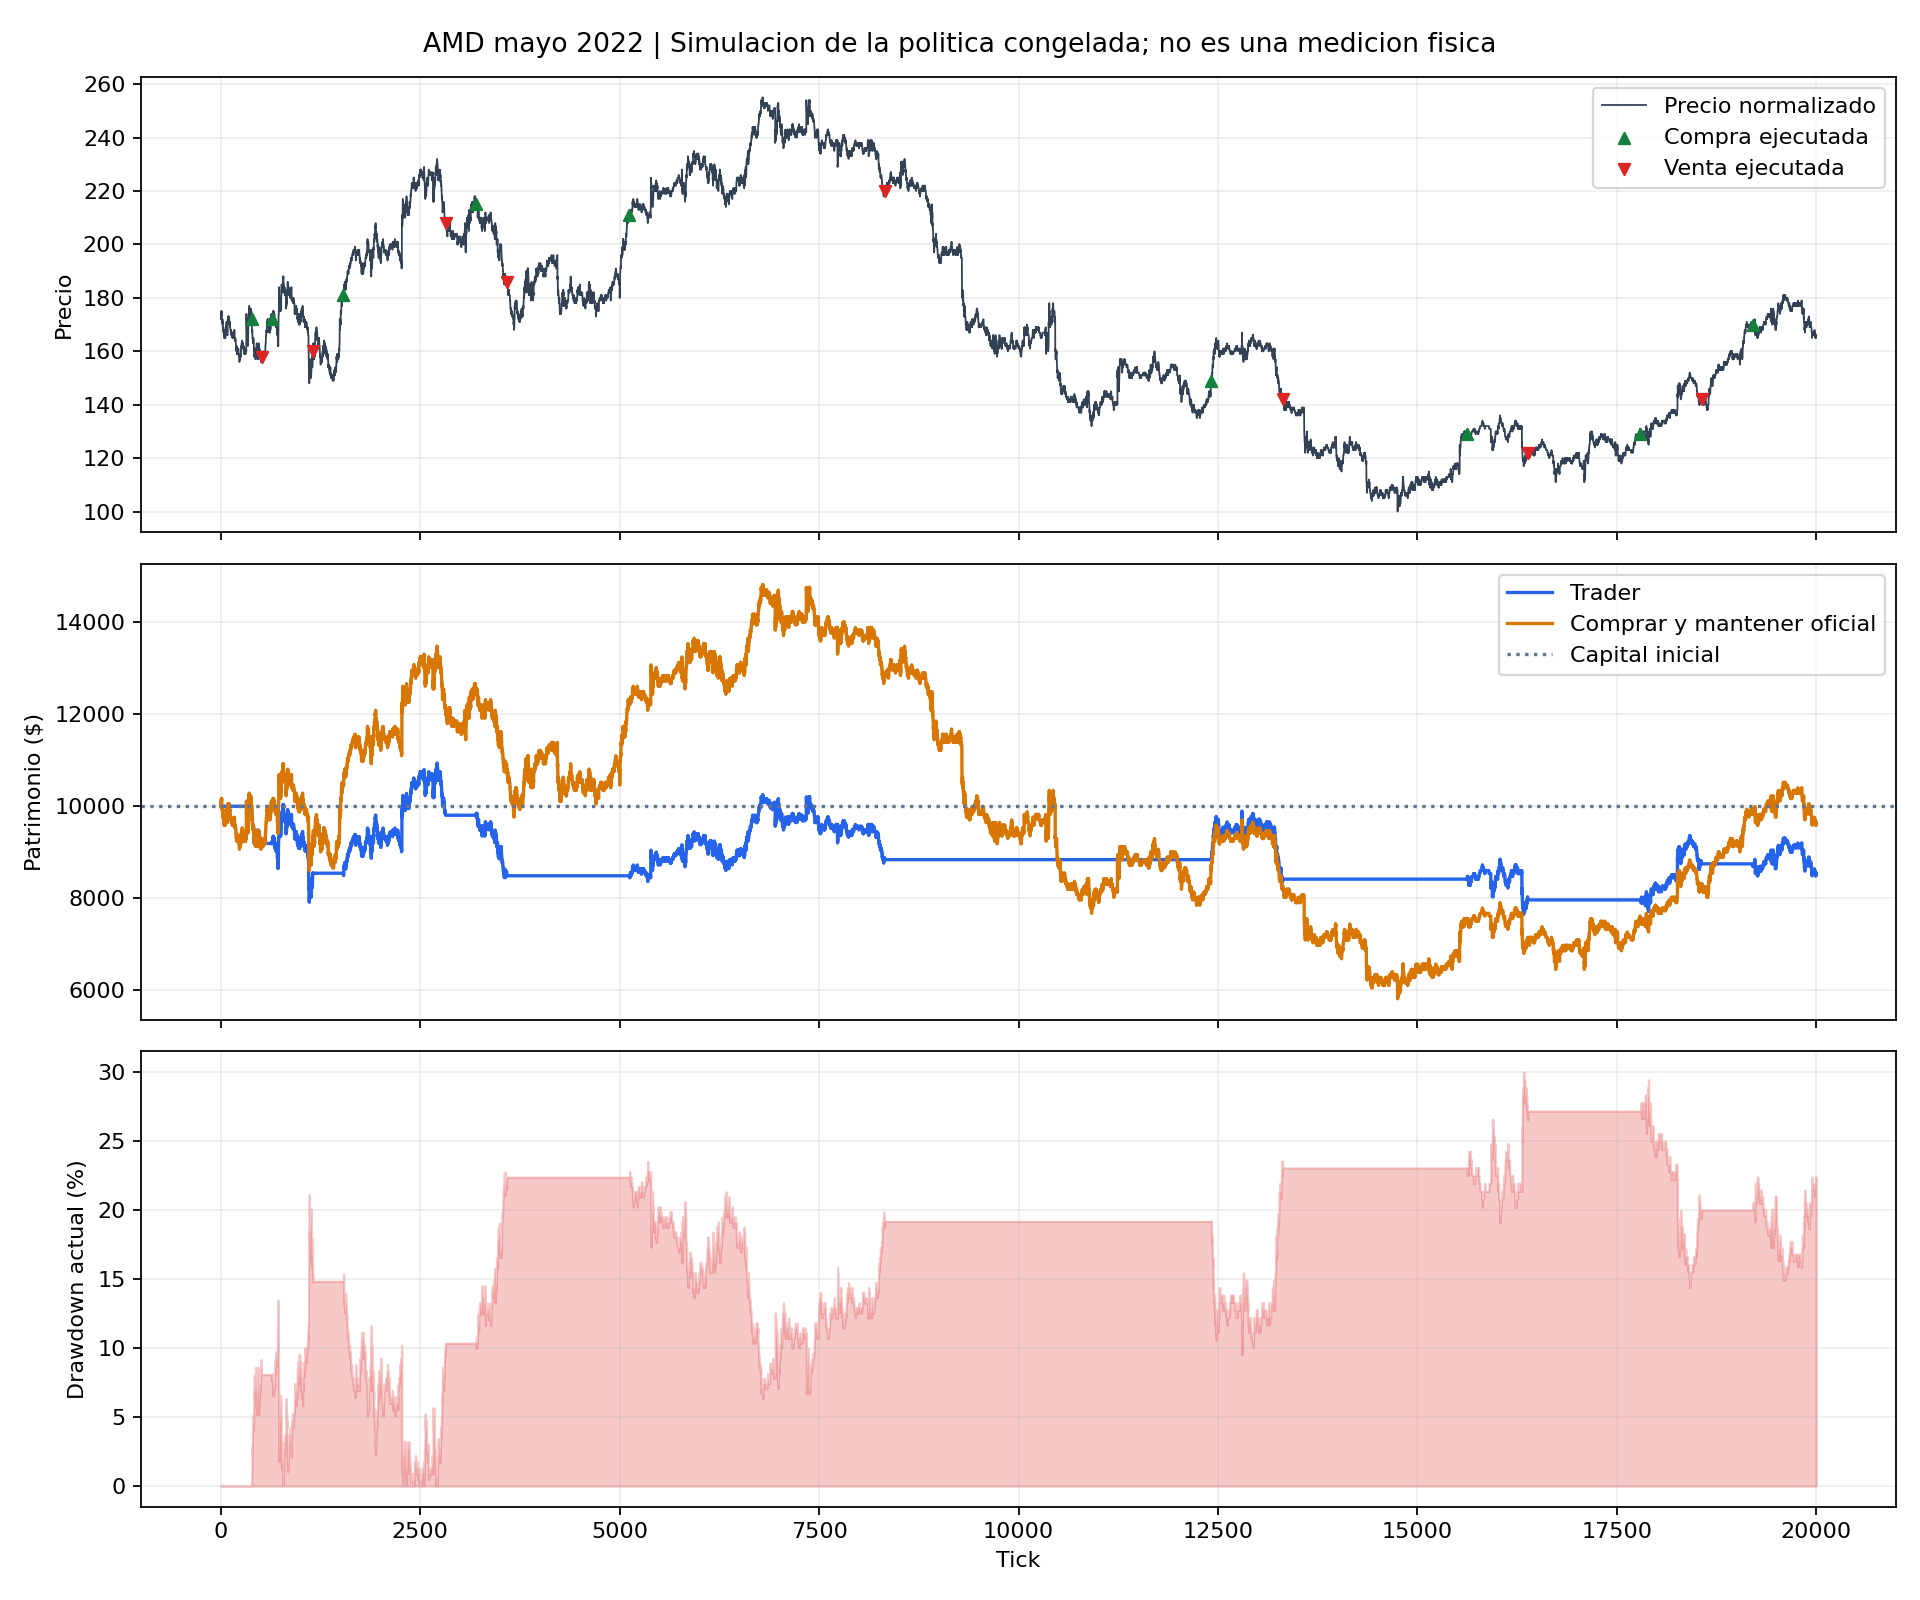
\includegraphics[width=\linewidth,height=0.70\textheight,keepaspectratio]{figuras/amd_mayo.png}\end{center}
Trader: \$8\,540; mantener: \$9\,647; ventaja: \$-1\,107. Órdenes: 17; comisiones: \$85; drawdown máximo: 30,01\%.

Los marcadores representan ejecuciones al precio siguiente al que generó la señal. Es simulación sobre datos conocidos; no es telemetría de la placa.

\clearpage\subsection{Apple 2022}
\begin{center}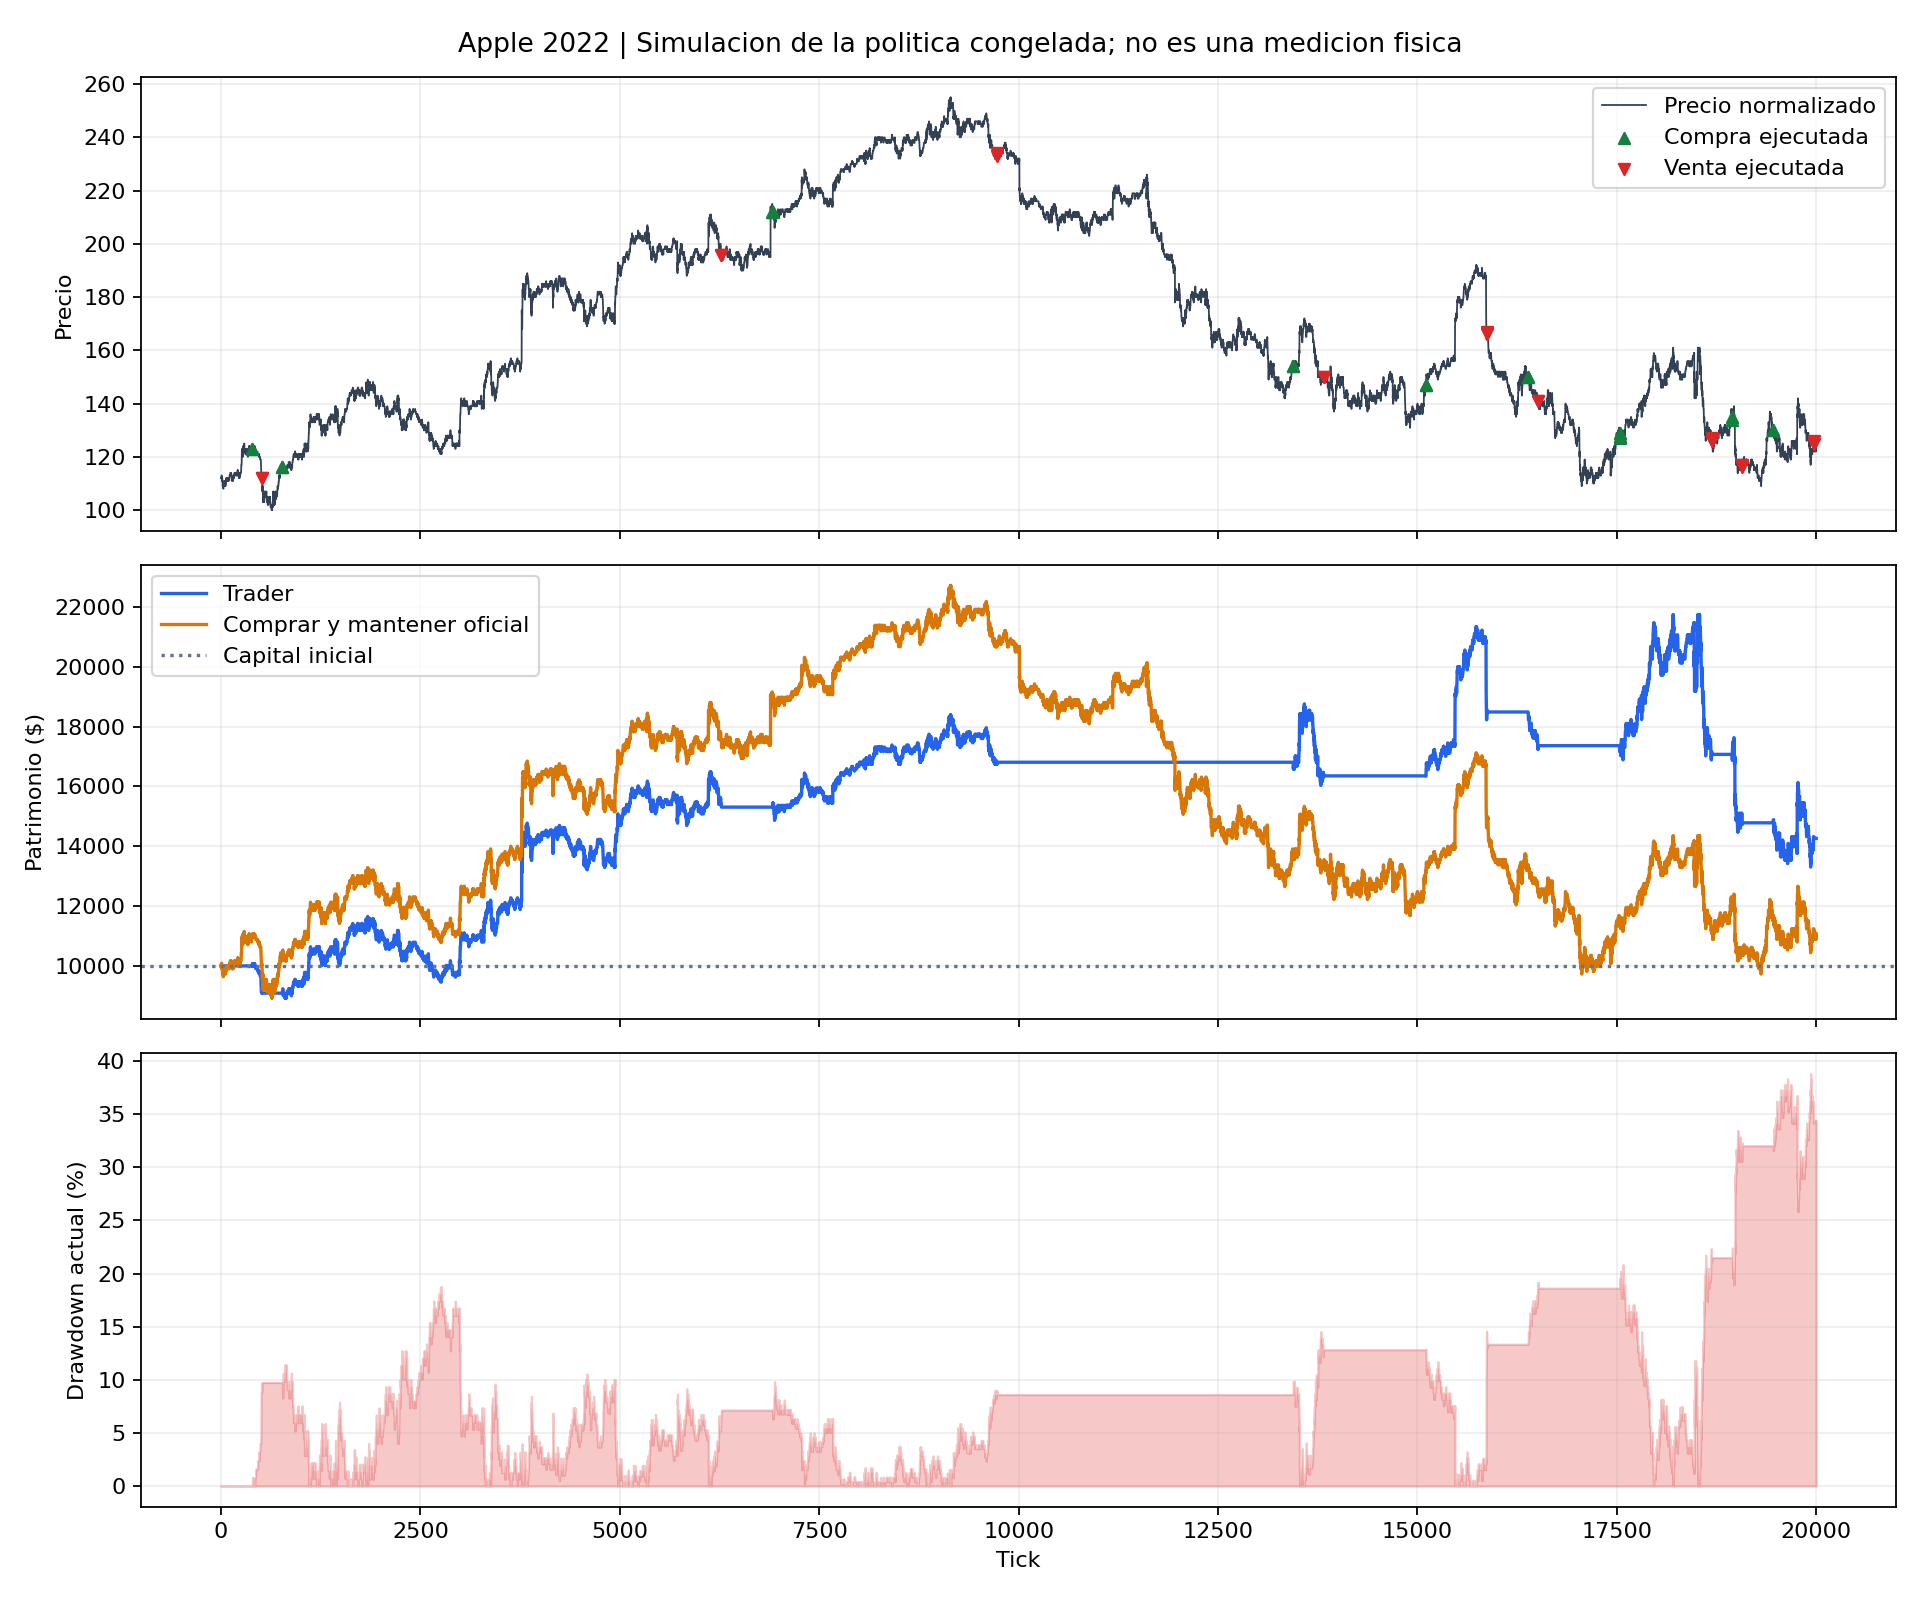
\includegraphics[width=\linewidth,height=0.70\textheight,keepaspectratio]{figuras/apple_2022.png}\end{center}
Trader: \$14\,263; mantener: \$11\,063; ventaja: \$3\,200. Órdenes: 38; comisiones: \$190; drawdown máximo: 38,82\%.

Los marcadores representan ejecuciones al precio siguiente al que generó la señal. Es simulación sobre datos conocidos; no es telemetría de la placa.

\clearpage\subsection{Apple 2023}
\begin{center}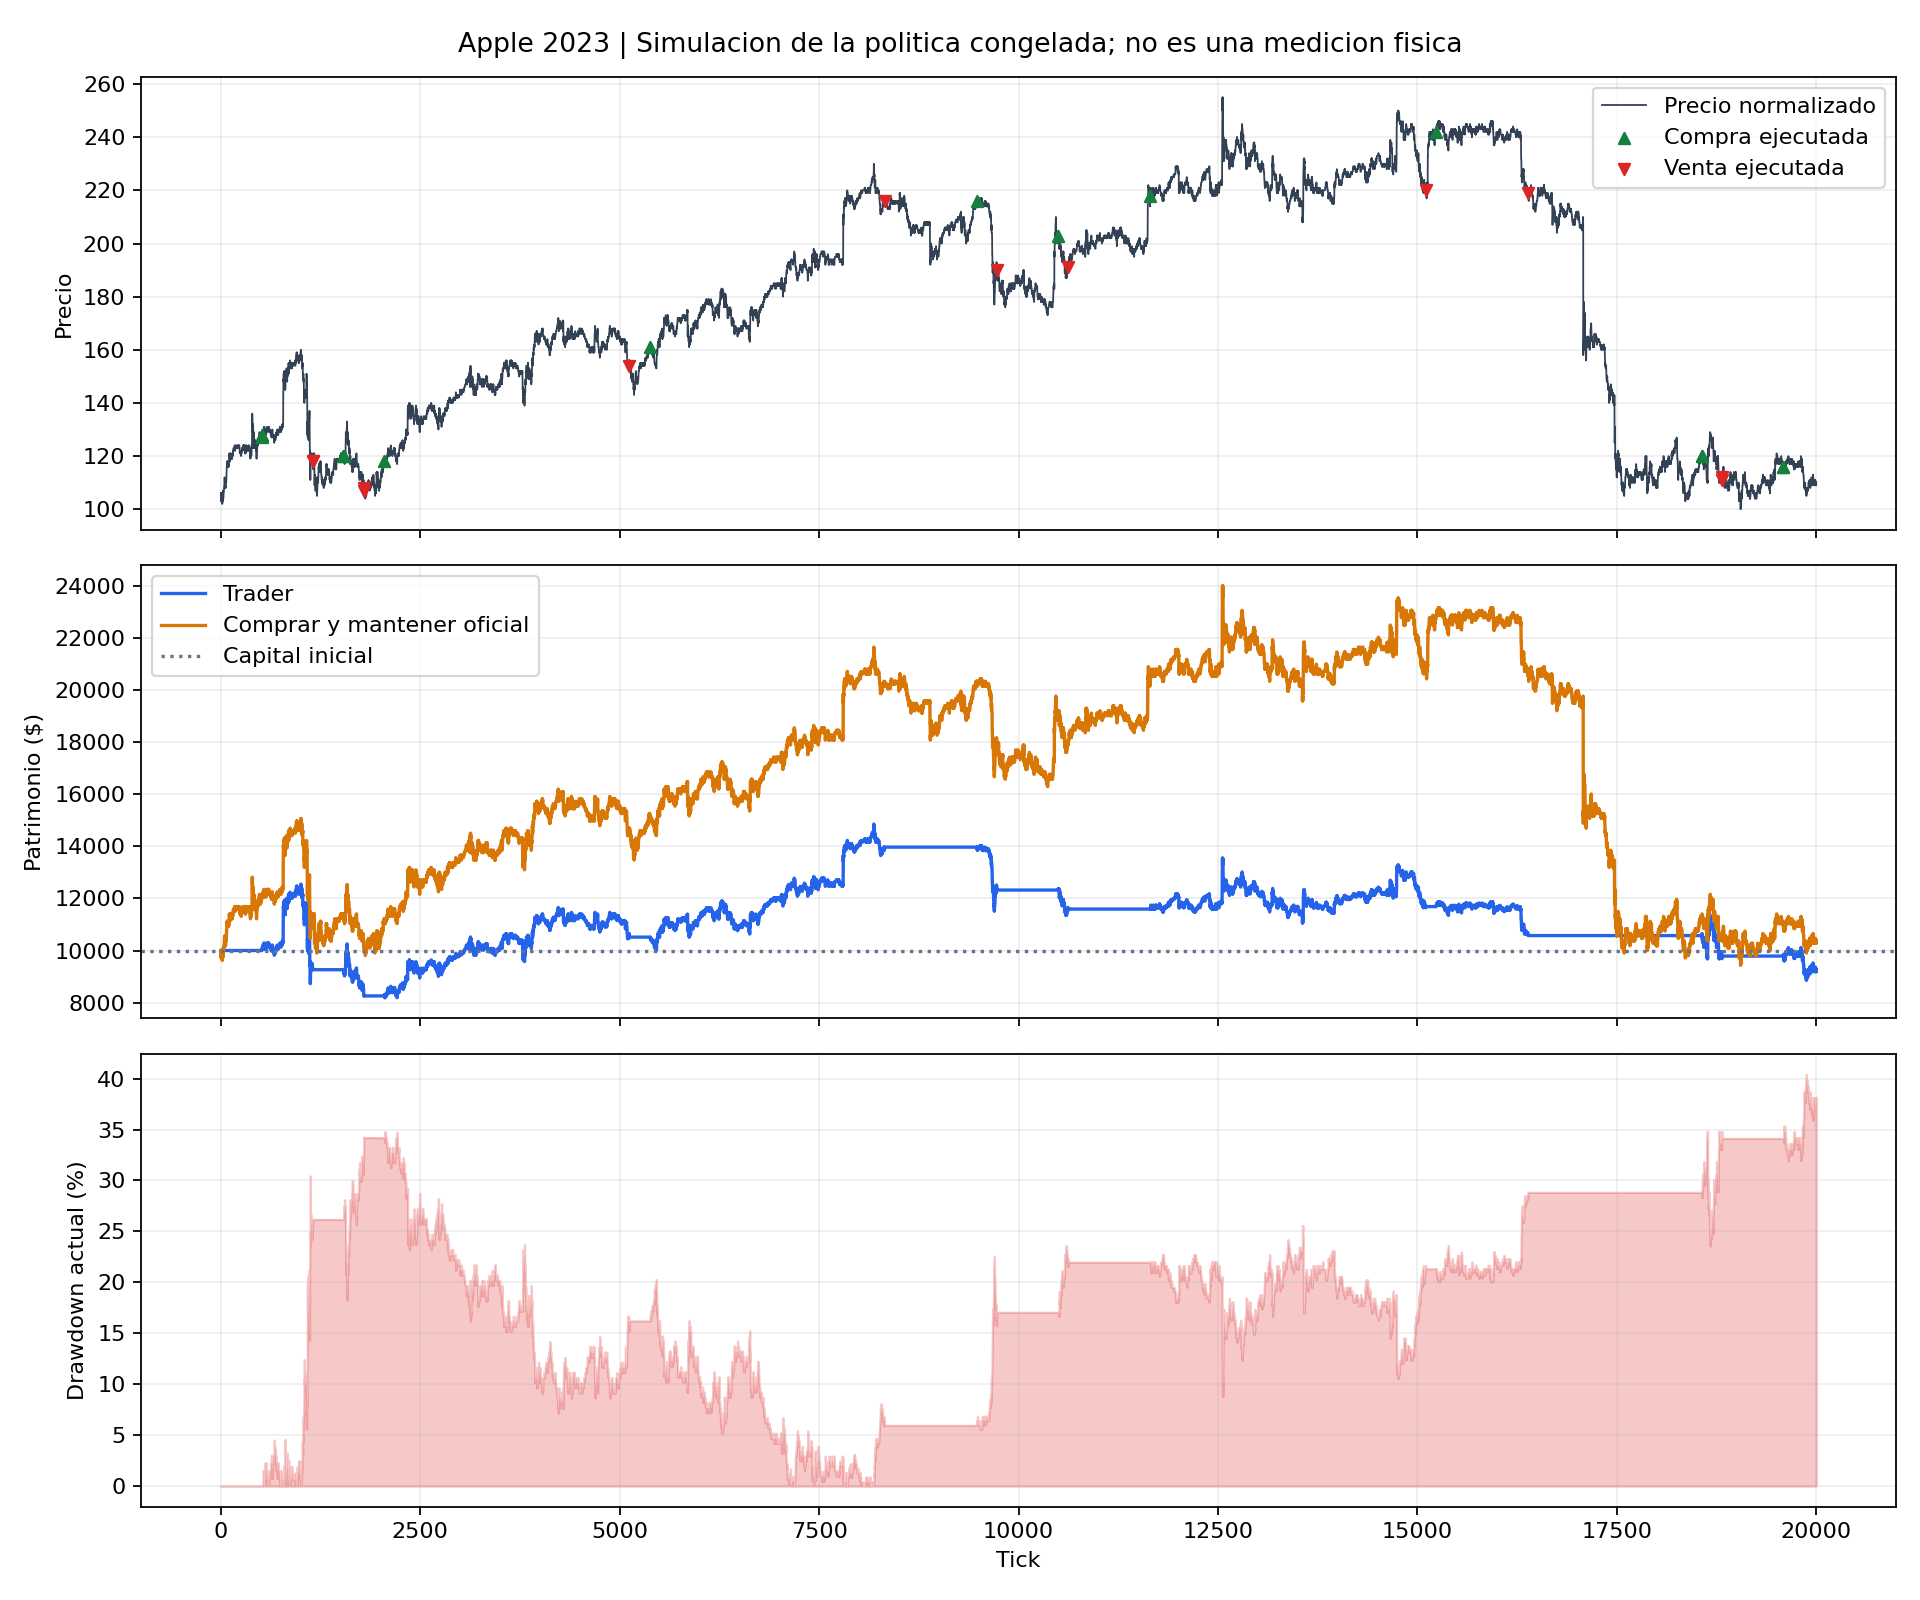
\includegraphics[width=\linewidth,height=0.70\textheight,keepaspectratio]{figuras/apple_2023.png}\end{center}
Trader: \$9\,272; mantener: \$10\,371; ventaja: \$-1\,099. Órdenes: 26; comisiones: \$130; drawdown máximo: 40,41\%.

Los marcadores representan ejecuciones al precio siguiente al que generó la señal. Es simulación sobre datos conocidos; no es telemetría de la placa.

\clearpage\subsection{Meta 2022}
\begin{center}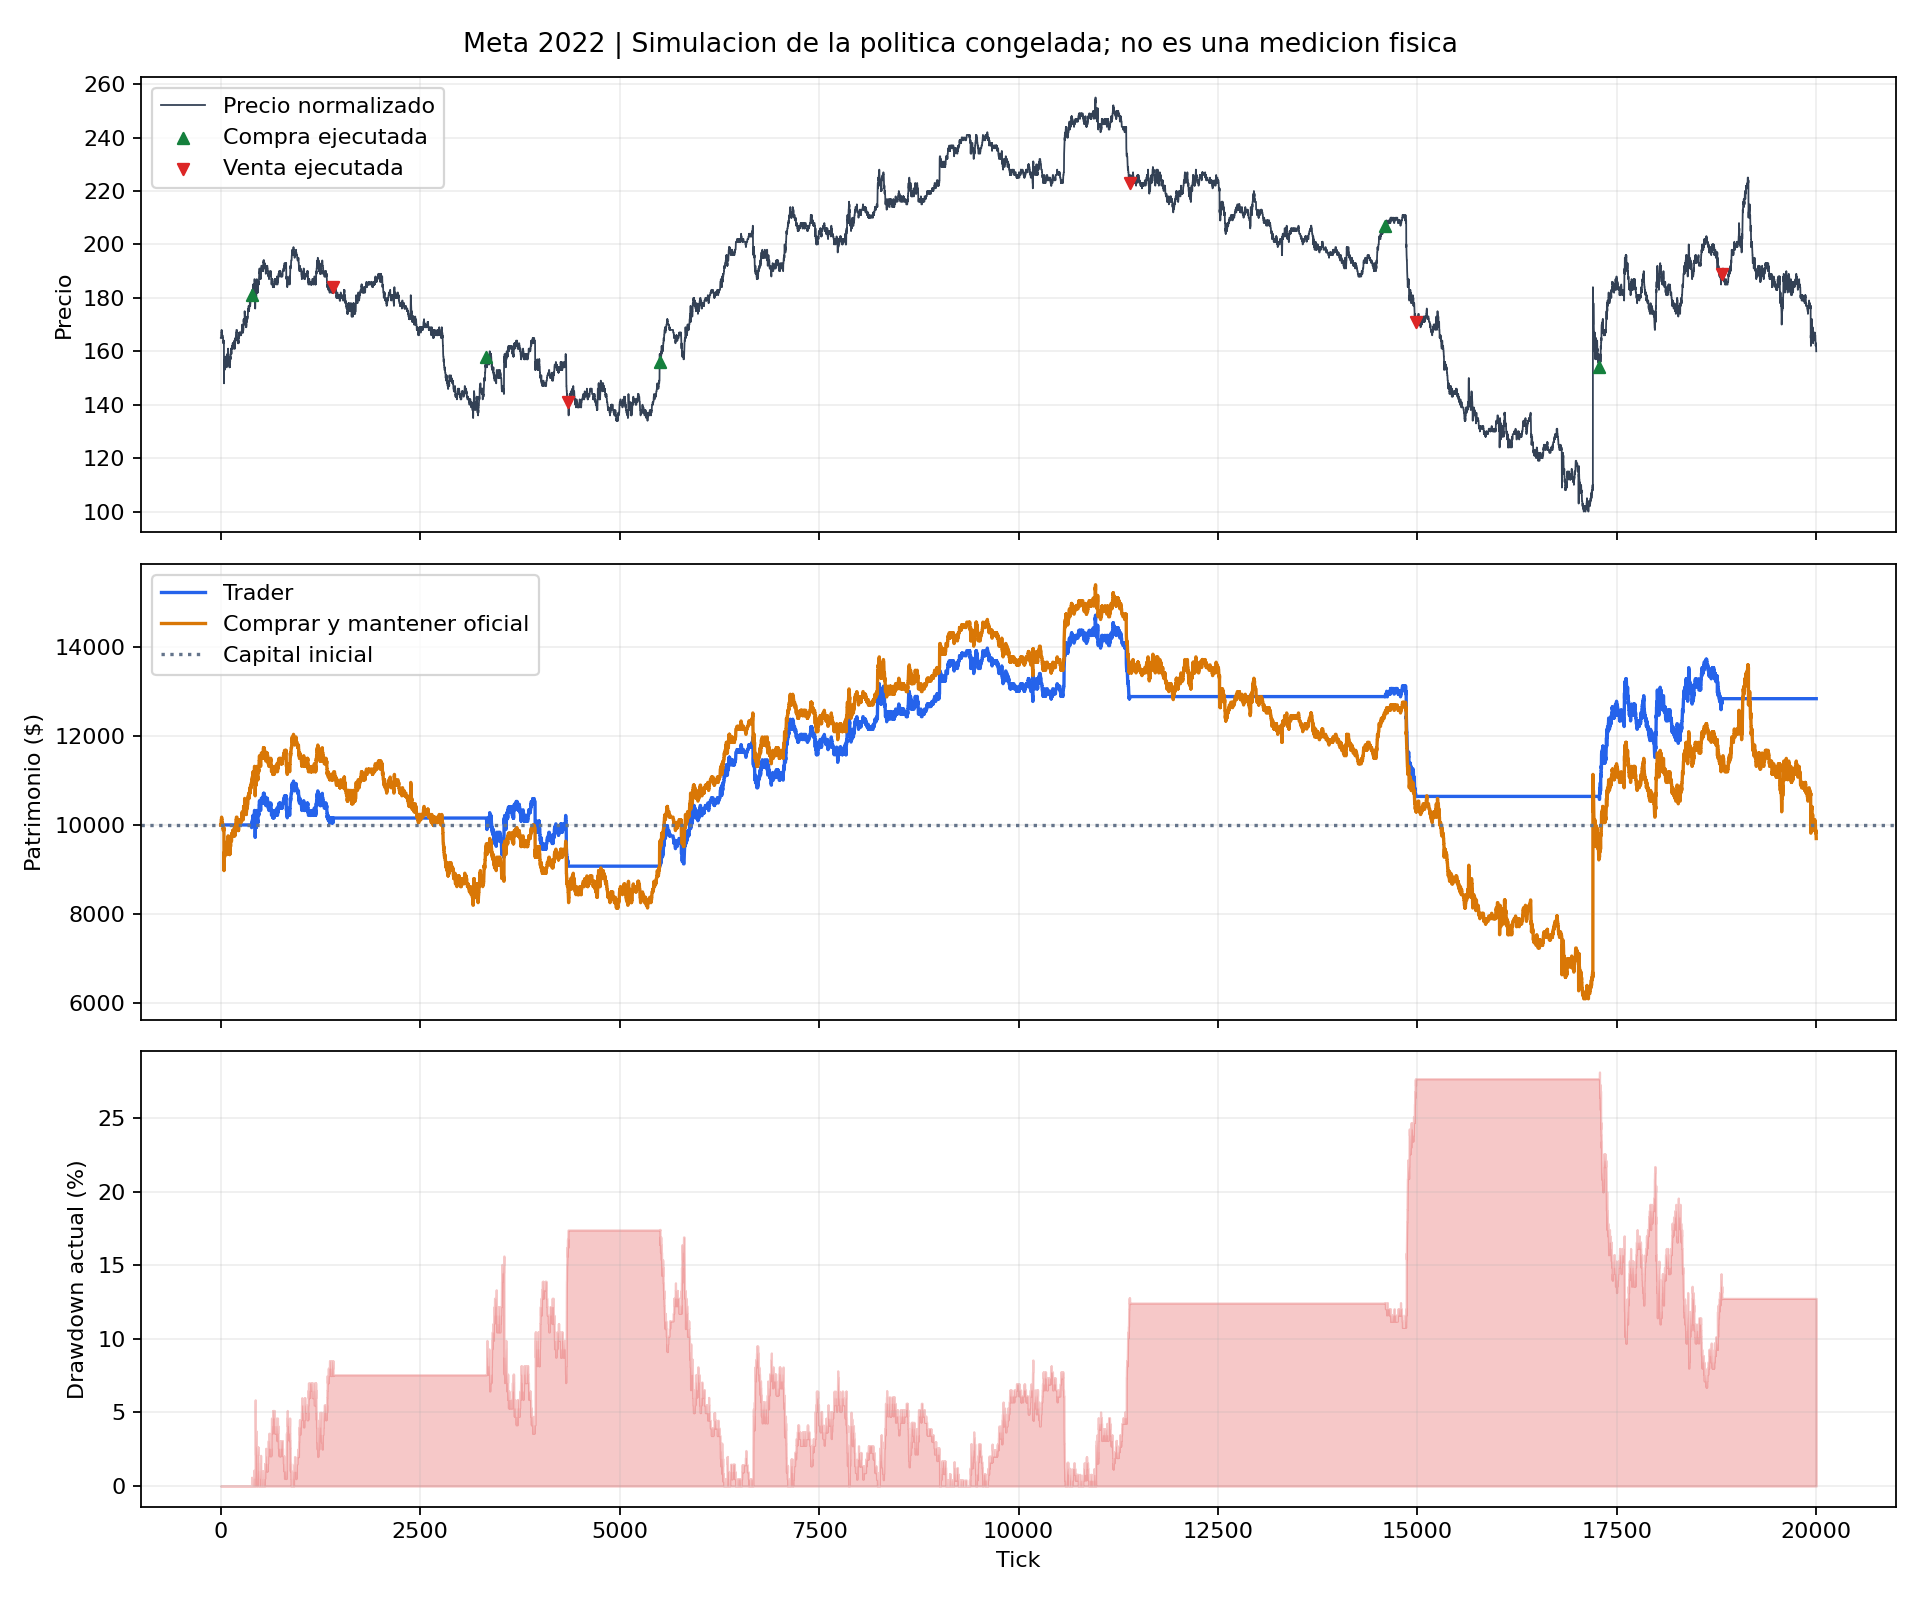
\includegraphics[width=\linewidth,height=0.70\textheight,keepaspectratio]{figuras/meta_2022.png}\end{center}
Trader: \$12\,836; mantener: \$9\,695; ventaja: \$3\,141. Órdenes: 10; comisiones: \$50; drawdown máximo: 28,13\%.

Los marcadores representan ejecuciones al precio siguiente al que generó la señal. Es simulación sobre datos conocidos; no es telemetría de la placa.

\clearpage\subsection{Netflix 2022}
\begin{center}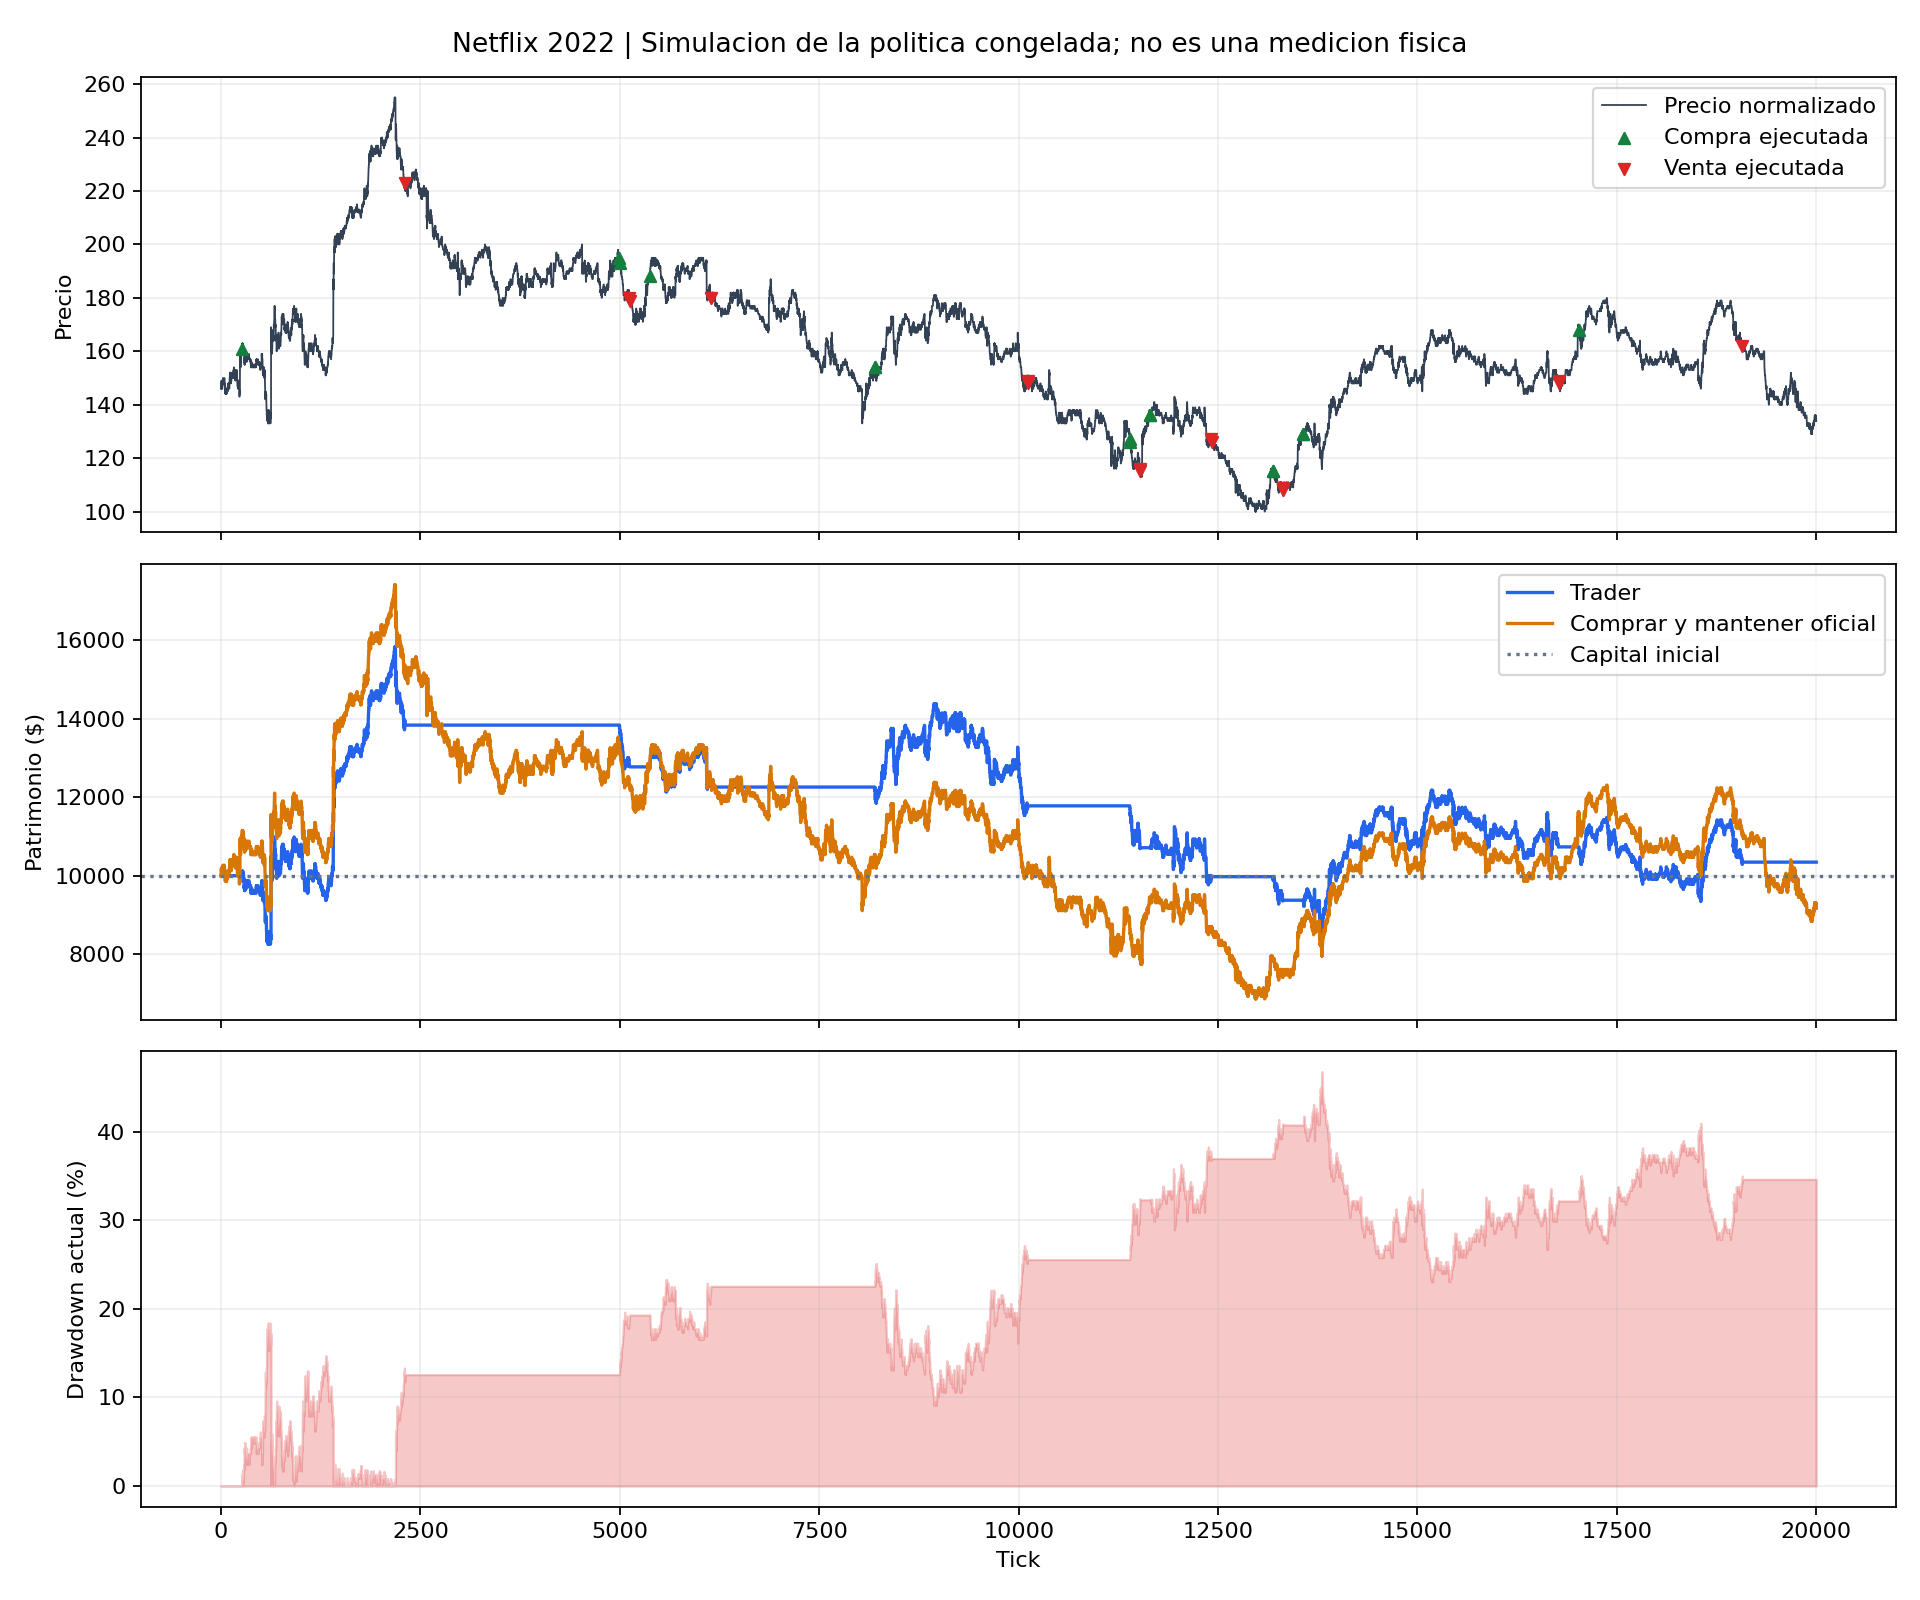
\includegraphics[width=\linewidth,height=0.70\textheight,keepaspectratio]{figuras/netflix_2022.png}\end{center}
Trader: \$10\,346; mantener: \$9\,179; ventaja: \$1\,167. Órdenes: 30; comisiones: \$150; drawdown máximo: 46,72\%.

Los marcadores representan ejecuciones al precio siguiente al que generó la señal. Es simulación sobre datos conocidos; no es telemetría de la placa.

\clearpage\subsection{Netflix 2023}
\begin{center}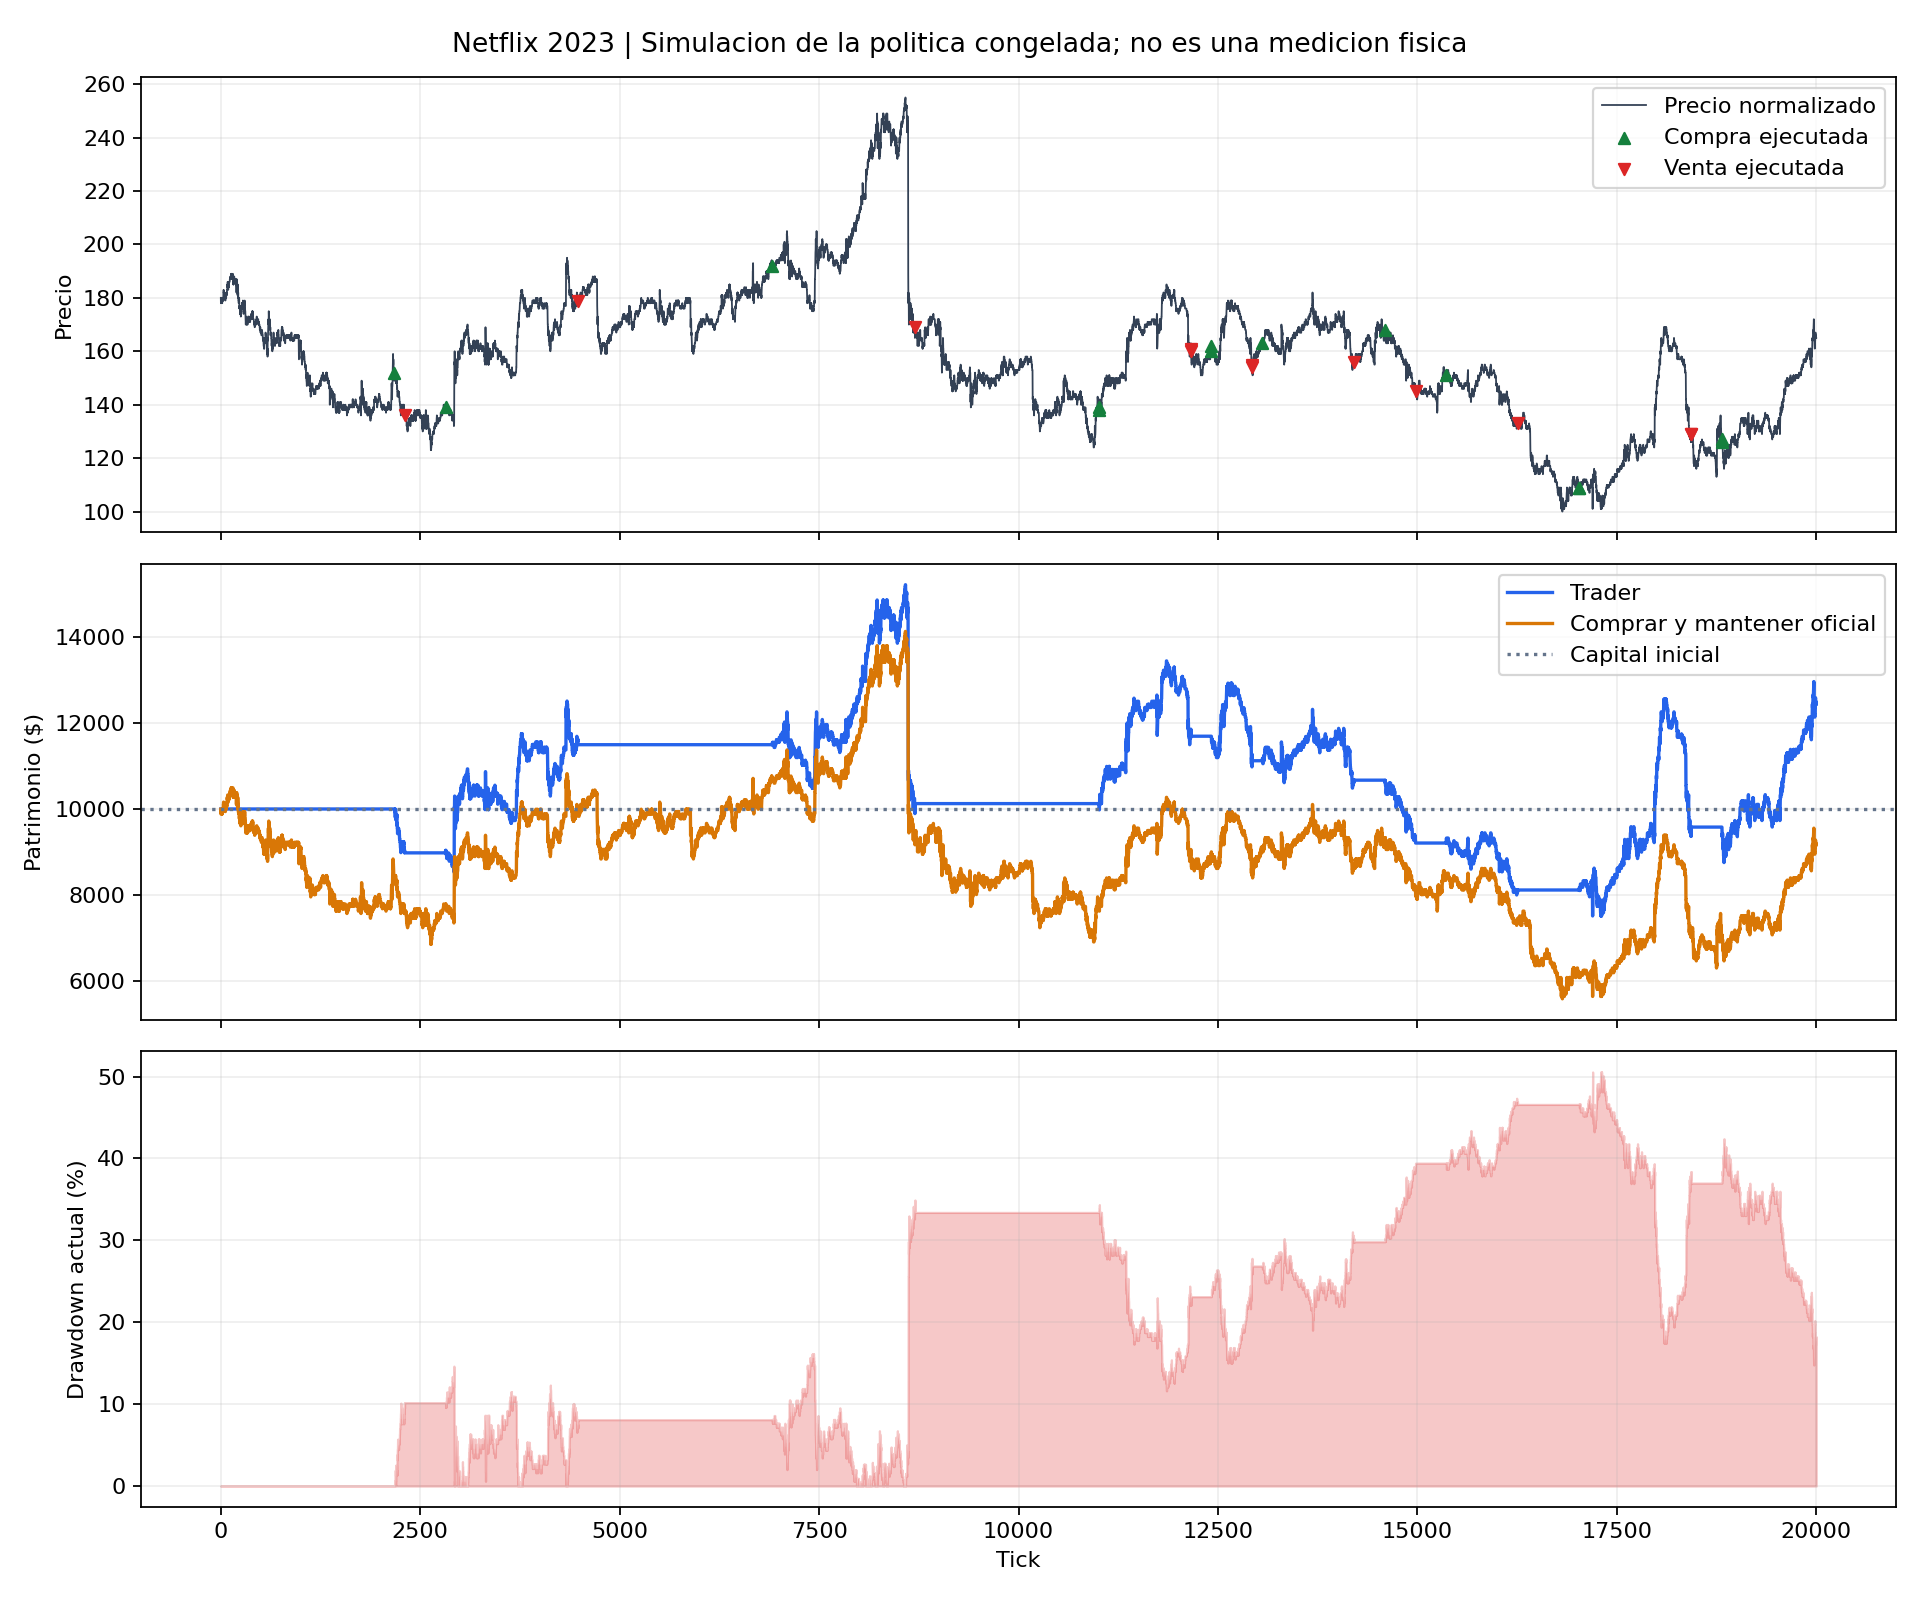
\includegraphics[width=\linewidth,height=0.70\textheight,keepaspectratio]{figuras/netflix_2023.png}\end{center}
Trader: \$12\,432; mantener: \$9\,170; ventaja: \$3\,262. Órdenes: 26; comisiones: \$130; drawdown máximo: 50,55\%.

Los marcadores representan ejecuciones al precio siguiente al que generó la señal. Es simulación sobre datos conocidos; no es telemetría de la placa.

\clearpage\subsection{Tesla 2022}
\begin{center}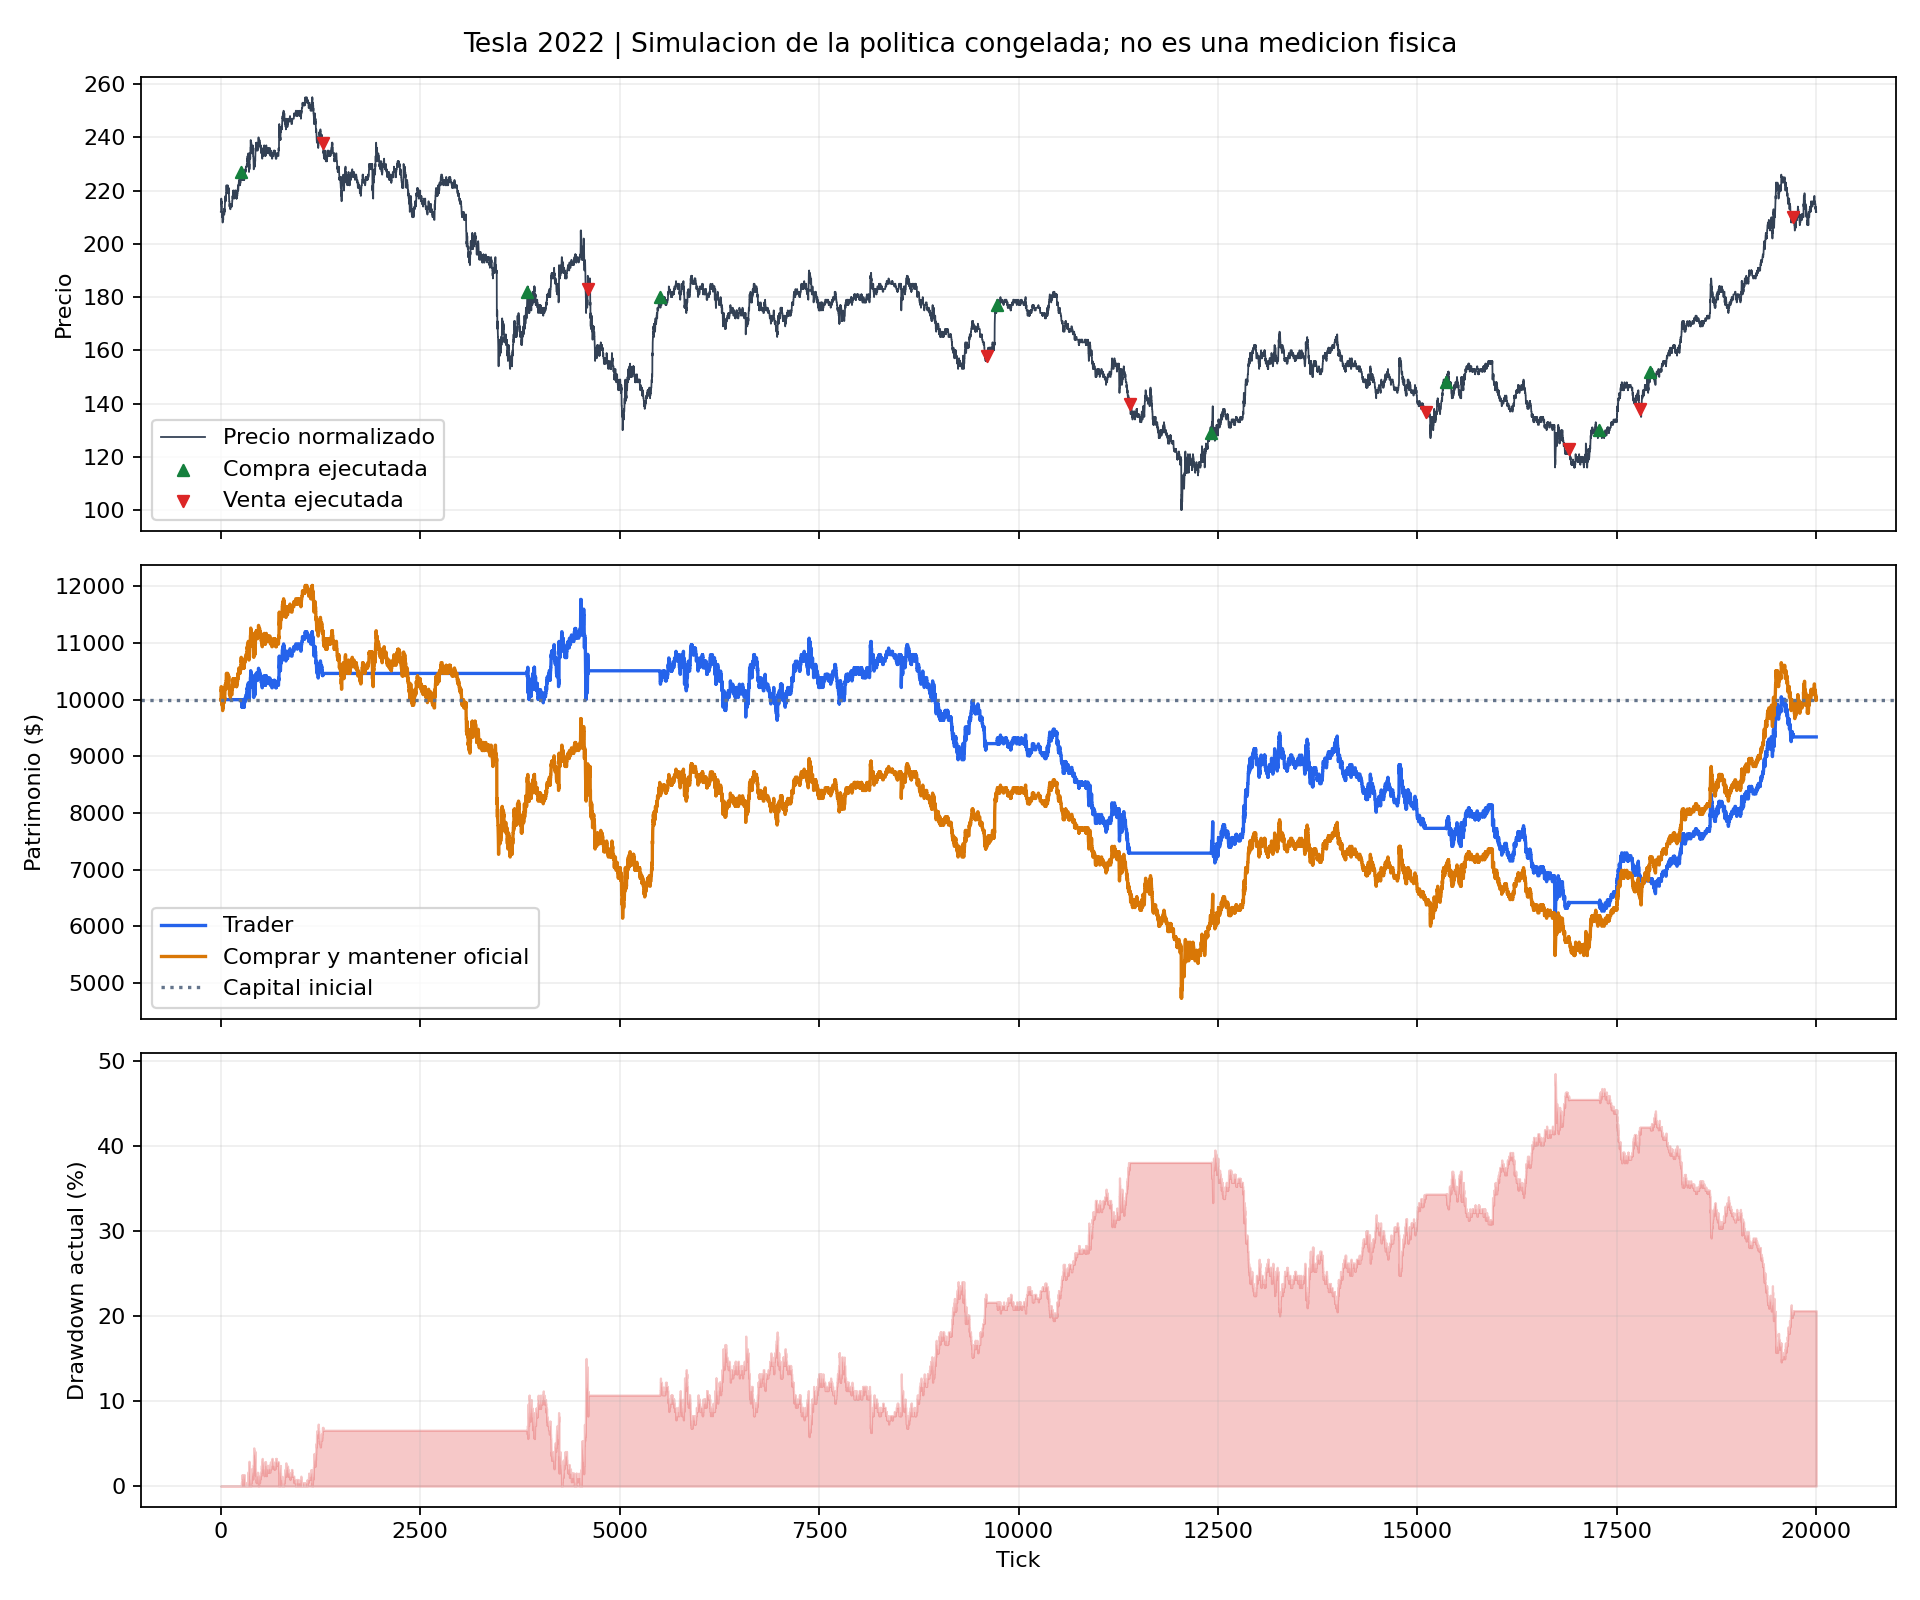
\includegraphics[width=\linewidth,height=0.70\textheight,keepaspectratio]{figuras/tesla_2022.png}\end{center}
Trader: \$9\,342; mantener: \$9\,995; ventaja: \$-653. Órdenes: 16; comisiones: \$80; drawdown máximo: 48,52\%.

Los marcadores representan ejecuciones al precio siguiente al que generó la señal. Es simulación sobre datos conocidos; no es telemetría de la placa.
